\documentclass[12pt, a4paper, oneside]{ctexart}
\usepackage{amsmath, amsthm, amssymb, bm, color, framed, graphicx, hyperref, mathrsfs}

\title{\textbf{10月27日作业}}
\author{韩岳成 524531910029}
\date{\today}
\linespread{1.5}
\definecolor{shadecolor}{RGB}{241, 241, 255}
\newcounter{problemname}
\newenvironment{problem}{\begin{shaded}\stepcounter{problemname}\par\noindent\textbf{题目\arabic{problemname}. }}{\end{shaded}\par}
\newenvironment{solution}{\par\noindent\textbf{解答. }}{\par}
\newenvironment{note}{\par\noindent\textbf{题目\arabic{problemname}的注记. }}{\par}

\begin{document}

\maketitle

\begin{problem}
    什么是维数灾难?请举例说明维数灾难可能带来的问题。
\end{problem}

\begin{solution}
    维数灾难是指在高维空间中,随着维度的增加,数据变得稀疏,导致计算复杂性和模型性能下降的问题。

    可能带来的问题:

    1. 在高维空间中,数据点直接的距离趋于相似,无法根据距离进行有效分类与计算。
    
    2. 需要更多的数据来填充高维空间,增加了数据收集和存储的成本。
    
    3. 计算复杂度增加,训练时间和资源消耗显著上升。
\end{solution}

\begin{problem}
    请绘制出$d=5,10,20$时$d$维球体体积$V(d)$随半径$r\in[0,1]$的变化曲线,分析维数$d$增大时的影响。
\end{problem}

\begin{solution}
    对于$d$维球体,其体积公式为:
    \[V(d, r) = \frac{\pi^{d/2}}{(d/2)!} r^d\]
    下面是$d=5,10,20$时,$V(d)$随$r\in[0,1]$的变化曲线:
   \begin{center}
    \begin{minipage}{0.48\textwidth}
        \centering
        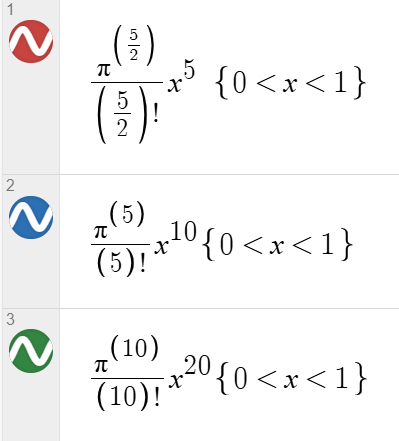
\includegraphics[width=\linewidth]{image-1.png}
    \end{minipage}\hfill
    \begin{minipage}{0.48\textwidth}
        \centering
        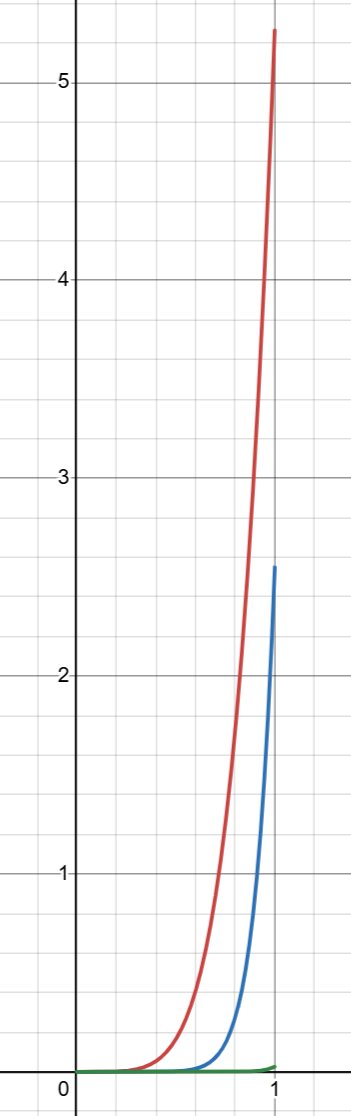
\includegraphics[width=\linewidth]{image-2.png}
    \end{minipage}
\end{center}

    随着维数$d$的增大,球体体积在$r$较小的范围内迅速减小,表明高维空间中球体的体积集中在边界附近。这进一步说明了维数灾难的问题,即数据在高维空间中变得稀疏,影响了模型的性能和计算效率。
\end{solution}

\begin{problem}
请证明蒙特卡洛方法的收敛阶是$O(n^{-\frac12})$,与维数 d 无关,即使采样数目 n 已经很大了。但我们前面在使用神经网络学习一个高维二次函数时在某些点的泛化误差依然很大,应该如何理解这个现象?
\end{problem}

\begin{solution}
由于期望具有线性性,
\[
\mathbb{E}[\hat{I}_n] = \frac{1}{n}\sum_{i=1}^n \mathbb{E}[f(X_i)] = \mathbb{E}[f(X)]
\]
因此 $\hat{I}_n$ 是无偏估计量。

利用独立性可得方差:
\[
\operatorname{Var}(\hat{I}_n) = \frac{1}{n^2}\sum_{i=1}^n \operatorname{Var}(f(X_i))
= \frac{\operatorname{Var}[f(X)]}{n}.
\]

因为 $\hat{I}_n$ 无偏,所以均方误差(MSE)即为其方差:
\[
\mathrm{MSE}(\hat{I}_n) = \mathbb{E}[(\hat{I}_n - \mu)^2] = \frac{\mathbb{E}[f(X)^2]}{n} - \left(\mathbb{E}[f(X)]\right)^2 = \frac{\operatorname{Var}[f(X)]}{n}.
\]

均方根误差(RMSE)为:
\[
\sqrt{\mathrm{MSE}} = \frac{\sqrt{\operatorname{Var}[f(X)]}}{\sqrt{n}} = O\left(n^{-1/2}\right).
\]

因此,蒙特卡洛方法的收敛阶为 $O(n^{-1/2})$。

某些点的泛化误差仍然很大的原因是:蒙特卡洛方法拟合的是标量期望,是一个全局意义上的误差,而我们想通过神经网络做的是函数拟合,是一个局部意义上的误差。即使全局误差很小,局部误差仍然可能很大。
由于高维空间中数据点非常稀疏,神经网络在某些区域可能没有足够的训练数据进行有效学习,导致这些区域的泛化误差较大。

\end{solution}
\end{document}